\documentclass[14pt,a4paper,article]{ncc}
\usepackage[a4paper, mag=1000, left=2.5cm, right=1cm, top=2cm, bottom=2cm, headsep=0.7cm, footskip=1cm]{geometry}
\usepackage[utf8]{inputenc}
\usepackage[T2A]{fontenc}
\usepackage[english,russian]{babel}
\usepackage{indentfirst}
%\usepackage[dvipsnames]{xcolor}
\usepackage[colorlinks]{hyperref}
\usepackage{amsfonts} 
\usepackage{amsmath}
\usepackage{graphicx}
\usepackage{float}
\graphicspath{{figure/}}
\DeclareGraphicsExtensions{.png,.jpg}

\usepackage{fancyhdr}
\pagestyle{fancy}
\fancyhead[LE,RO]{\thepage}
\fancyfoot{}

\usepackage{listings}

\hypersetup{linkcolor=black}


\begin{document}
% Title page 
\begin{titlepage}
    \begin{center}
        \textsc{
            Санкт-Петербургский политехнический университет имени Петра Великого \\[5mm]
            Физико-механический институт\\[2mm]
            Высшая школа прикладной математики и физики            
        }   
        \vfill
        \textbf{\large
            Отчет по лаборабороной работу №1\\
            по дисциплине "Интервальный анализ"\\[3mm]
        }                
    \end{center}

    \vfill
    \hfill
    \begin{minipage}{0.5\textwidth}
        Выполнил: \\[2mm]   
		Студент: Габдушев Рушан \\
		Группа: 5030102/90201\\
    \end{minipage}

	\hfill
	\begin{minipage}{0.5\textwidth}
		Принял: \\[2mm]
		к. ф.-м. н., доцент \\   
		Баженов Александр Николаевич
	\end{minipage}

    \vfill
    \begin{center}
        \theyear\ г.
    \end{center}
\end{titlepage}

\tableofcontents
\newpage
\listoffigures
\newpage
\listoftables
\newpage

\section{Постановка задачи}
\subsection{Задача 2: поиск глобального минимума}

Для функции Бута (Booth's function)
\begin{equation}
	f(x, y) = (x + 2y - 7)^{2} + (2x + y - 5)^{2} 
\end{equation}
имеющей один глобальный экстремум, и функции Химмельблау
\begin{equation}
	f(x, y) = (x^{2} + y - 11)^{2} + (x + y^{2} - 7)^{2} 
\end{equation}
имеющей 4 равнозначных глобальных экстремума, необходимо провести вычисления по поиску глобального минимума с помощью простейшего интервального адаптивного алгоритма глобальной оптимизации.
\subsection{Задача 2: поиск глобального минимума}

Для функции Бута (Booth's function)
\begin{equation}
	f(x, y) = (x + 2y - 7)^{2} + (2x + y - 5)^{2} 
\end{equation}
имеющей один глобальный экстремум, и функции Химмельблау
\begin{equation}
	f(x, y) = (x^{2} + y - 11)^{2} + (x + y^{2} - 7)^{2} 
\end{equation}
имеющей 4 равнозначных глобальных экстремума, необходимо провести вычисления по поиску глобального минимума с помощью простейшего интервального адаптивного алгоритма глобальной оптимизации.
\newpage

\section{Теория}
\subsection{Критерий Баумана}
Матрица \textbf{A} $\in {\mathbb{R}}^{n \times n}$ неособенна \Leftrightarrow \forall A', A'' $\in$ vert \textbf{A} det(A') · det(A'') > 0 

\subsection{Глобальная оптимизация}
Суть простейшего интервального адаптивного алгоритма глобальной оптимизации похожа на алгоритм дихотомии, только для многомерного случая. Имеется рабочий список рассматриваемых брусьев, для каждого из которых вычислено целевое значение функции (в интервальном смысле). На каждой итерации метод выбирает из этого списка брус, на котором нижняя оценка значения функции наименьшая. Этот брус удаляется из списка, после чего туда добавляются два новых, которые получились из исходного путем дробления его самой длинной компоненты пополам (от нижней границы до середины и от середины до верхней границы). На этих брусьях вычисляется интервальная оценка целевой функции, выполняется переход на новую итерацию.

\newpage

\section{Реализация}
Данная лабораторная работа была выполнена с использованием языка
программирования Python 3.10 в среде разработки Visual Studio Code с
использованием следующих библиотек:
\begin{itemize}
\item intvalpy версии 1.5.8
\item numpy версии 1.22.0
\item matplotlib версии 3.5.1
\end{itemize}

\newpage

\section{Результаты}
\subsection{Задача 2: поиск глобального минимума}

\subsubsection{функция с одним глобальным минимумом}

\begin{figure}[H]
		\centering
			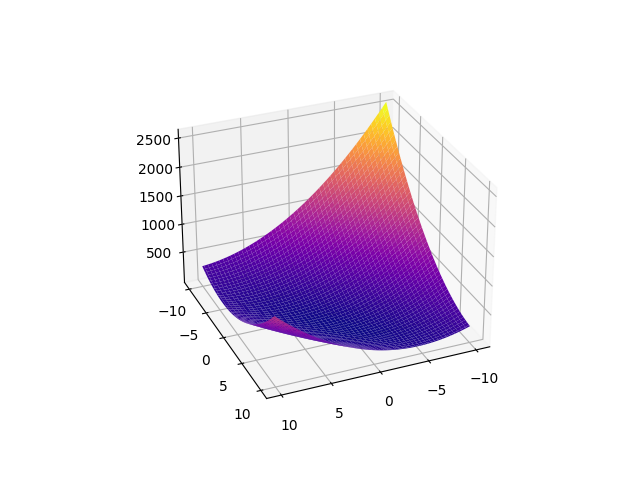
\includegraphics{task2/resources/Figure_1.png}
		\caption{График функции Бута}
		\label{w_pert}
	\end{figure}

Рассматриваемая функция Бута $f(x, y)$ имеет один глобальный минимум. Заранее известны точка минимума и значение функции в ней:

\begin{table}[H]
	\centering
	\begin{tabular}{| c | c | c |}
		\hline
		    x_{min} & y_{min} & f(x_{min}, y_{min}) \\
		\hline
		    1 & 3 & 0 \\
   		\hline
	\end{tabular}
	\caption{Все точки минимумов функции Бута и их значения}
\end{table}

Рассмотрим работу алгоритма поиска глобального минимума на начальном брусе \textbf{A} = [(-10, 10), (-10, 10)], $\epsilon = 0.01$. Черная линия - путь работы алгоритма, красная точка - найденный алгоритмом глобальный минимум.

\begin{figure}[H]
	\centering
		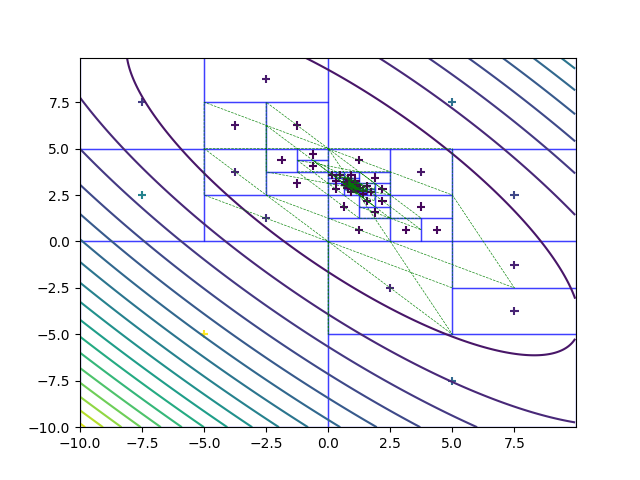
\includegraphics{task2/resources/Figure_2.png}
	\caption{Поиск глобального минимума функции Бута}
	\label{w_pert}
\end{figure}

\begin{table}[H]
	\centering
	\begin{tabular}{| c | c | c |}
		\hline
		    x* & y* & f(x*, y*) \\
		\hline
		    1.025390625 & 2.98828125 & 0 \\
   		\hline
	\end{tabular}
	\caption{Найденный алгоритмом глобальный минимум функции Бута}
\end{table}

\newpage
\subsubsection{Функция с несколькими глобальными минимумами}

\begin{figure}[H]
		\centering
			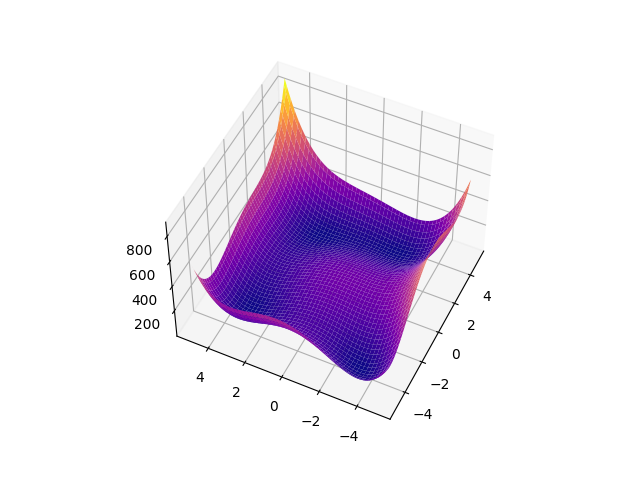
\includegraphics{task2/resources/Figure_3.png}
		\caption{График функции Химмельблау}
		\label{w_pert}
	\end{figure}

Рассматриваемая функция Химмельблау $f(x, y)$ имеет четыре глобальных минимума. Заранее известны точки минимумы и значения функций в ней:

\begin{table}[H]
	\centering
	\begin{tabular}{| c | c | c |}
		\hline
		    x_{min} & y_{min} & f(x_{min}, y_{min}) \\
		\hline
		    3 & 2 & 0 \\
		    -2.805118 & 3.131312 & 0 \\
		    -3.779310 & -3.283186 & 0 \\
		    3.584428 & -1.848126 & 0 \\
   		\hline
	\end{tabular}
	\caption{Все точки минимумов функции Химмельблау и их значения}
\end{table}

Рассмотрим работу алгоритма поиска глобального минимума на начальном брусе \textbf{A} = [(-5, 5), (-5, 5)], $\epsilon = 0.01$. Черная линия - путь работы алгоритма, красная точка - найденный алгоритмом глобальный минимум.

\begin{figure}[H]
	\centering
		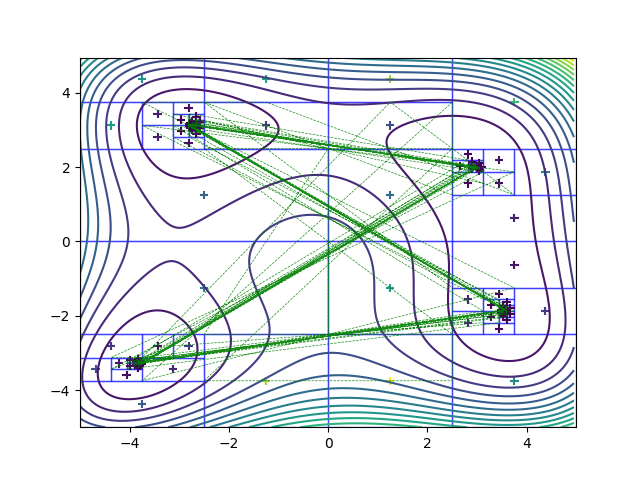
\includegraphics{task2/resources/Figure_4.png}
	\caption{Поиск глобального минимума функции Химмельблау}
	\label{w_pert}
\end{figure}

\begin{table}[H]
	\centering
	\begin{tabular}{| c | c | c |}
		\hline
		    x* & y* & f(x*, y*) \\
		\hline
		    2.998046875 & 2.001953125 & 0 \\
   		\hline
	\end{tabular}
	\caption{Найденный алгоритмом глобальный минимум функции Химмельблау}
\end{table}

\subsection{Задача 2: поиск глобального минимума}

\subsubsection{функция с одним глобальным минимумом}

\begin{figure}[H]
		\centering
			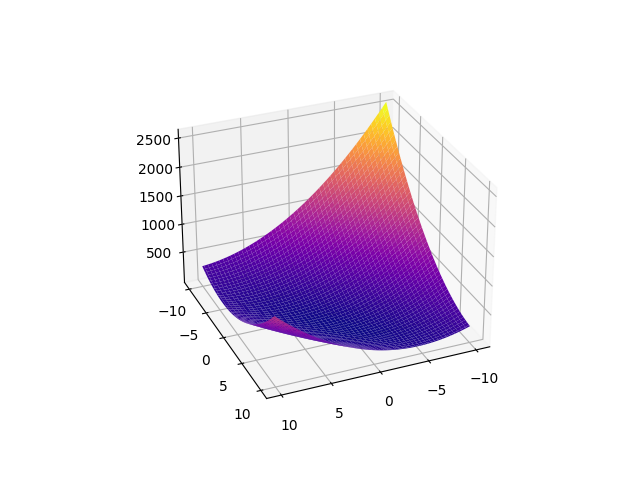
\includegraphics{task2/resources/Figure_1.png}
		\caption{График функции Бута}
		\label{w_pert}
	\end{figure}

Рассматриваемая функция Бута $f(x, y)$ имеет один глобальный минимум. Заранее известны точка минимума и значение функции в ней:

\begin{table}[H]
	\centering
	\begin{tabular}{| c | c | c |}
		\hline
		    x_{min} & y_{min} & f(x_{min}, y_{min}) \\
		\hline
		    1 & 3 & 0 \\
   		\hline
	\end{tabular}
	\caption{Все точки минимумов функции Бута и их значения}
\end{table}

Рассмотрим работу алгоритма поиска глобального минимума на начальном брусе \textbf{A} = [(-10, 10), (-10, 10)], $\epsilon = 0.01$. Черная линия - путь работы алгоритма, красная точка - найденный алгоритмом глобальный минимум.

\begin{figure}[H]
	\centering
		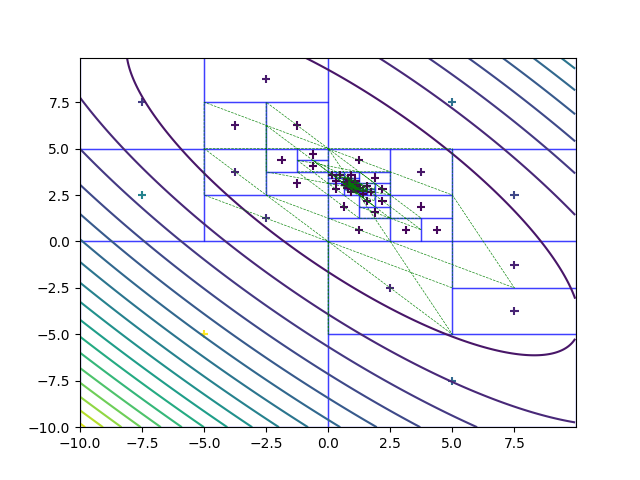
\includegraphics{task2/resources/Figure_2.png}
	\caption{Поиск глобального минимума функции Бута}
	\label{w_pert}
\end{figure}

\begin{table}[H]
	\centering
	\begin{tabular}{| c | c | c |}
		\hline
		    x* & y* & f(x*, y*) \\
		\hline
		    1.025390625 & 2.98828125 & 0 \\
   		\hline
	\end{tabular}
	\caption{Найденный алгоритмом глобальный минимум функции Бута}
\end{table}

\newpage
\subsubsection{Функция с несколькими глобальными минимумами}

\begin{figure}[H]
		\centering
			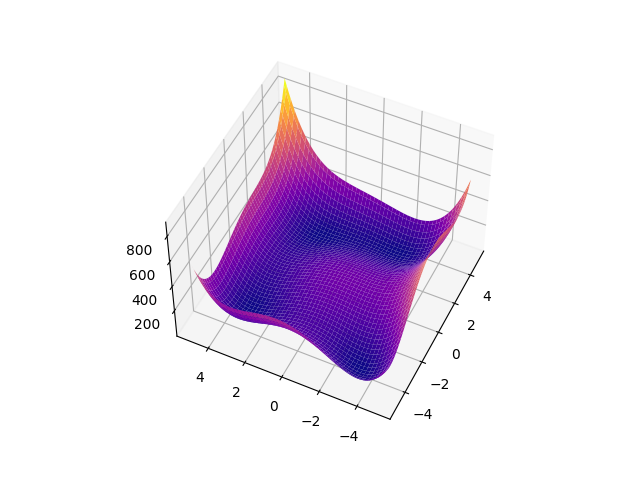
\includegraphics{task2/resources/Figure_3.png}
		\caption{График функции Химмельблау}
		\label{w_pert}
	\end{figure}

Рассматриваемая функция Химмельблау $f(x, y)$ имеет четыре глобальных минимума. Заранее известны точки минимумы и значения функций в ней:

\begin{table}[H]
	\centering
	\begin{tabular}{| c | c | c |}
		\hline
		    x_{min} & y_{min} & f(x_{min}, y_{min}) \\
		\hline
		    3 & 2 & 0 \\
		    -2.805118 & 3.131312 & 0 \\
		    -3.779310 & -3.283186 & 0 \\
		    3.584428 & -1.848126 & 0 \\
   		\hline
	\end{tabular}
	\caption{Все точки минимумов функции Химмельблау и их значения}
\end{table}

Рассмотрим работу алгоритма поиска глобального минимума на начальном брусе \textbf{A} = [(-5, 5), (-5, 5)], $\epsilon = 0.01$. Черная линия - путь работы алгоритма, красная точка - найденный алгоритмом глобальный минимум.

\begin{figure}[H]
	\centering
		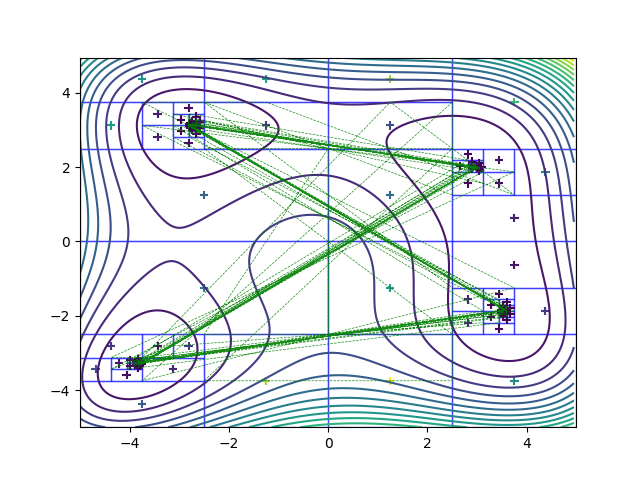
\includegraphics{task2/resources/Figure_4.png}
	\caption{Поиск глобального минимума функции Химмельблау}
	\label{w_pert}
\end{figure}

\begin{table}[H]
	\centering
	\begin{tabular}{| c | c | c |}
		\hline
		    x* & y* & f(x*, y*) \\
		\hline
		    2.998046875 & 2.001953125 & 0 \\
   		\hline
	\end{tabular}
	\caption{Найденный алгоритмом глобальный минимум функции Химмельблау}
\end{table}

\newpage

\section{Обсуждение}
\subsection{Поиск $\delta$}

Рассмотренная нами матрица является неособенной при малых значения $\delta$. Матрица становятся особенными, когда интервалы, находящиеся в столбцах, имеют не пустое пересечение. Более того, если происходит пересечение интервалов во всех столбцах определенных строк, то тогда можно выделить такую точечную матрицу, из этих интервалов, в которой определитель будет равен 0. Иначе говоря, в таком случае определитель матрицы интервалов содержит в себе 0.

\subsection{Поиск глобального минимума}

Для обеих функций алгоритм нахождения минимума функции дал правильную оценку значения минимума функции, при этом чуть хуже оценил аргументы, сообщающие минимум. При этом видно, что для функции, имеющей несколько равнозначных глобальных минимумов наблюдаются скачки между этими самыми локальными минимумами. Скачкообразное поведение графиков объясняется самим алгоритмом: ведущий брус, который будет далее дробиться, выбирается на каждой итерации путем полного итерирования по рабочему списку, то есть не обязательно последний брус дает наилучшее приближение к минимуму.
\newpage

\section{Ссылки на библиотеки}
\begin{enumerate}
\item \url{https://pypi.org/project/intvalpy/} \ - intvalpy
\item \url{https://numpy.org/} \ - NumPy
\item \url{https://matplotlib.org/stable/index.html} \ - Matplotlib
\end{enumerate}
\newpage

\section{Ссылки на репозиторий}
\url{https://github.com/AS2/interval_analysis} \ - GitHub репозиторий

\end{document}